%%%%%%%%%%%%%%%%%%%%%%%%%%%%%%%%%%%%%%%%%%%%%%%%%%%%%%%%%%%%%%%%%%%%%%%%
%                                                                      %
%     File: Thesis_Background.tex                                      %
%     Tex Master: Thesis.tex                                           %
%                                                                      %
%     Author: Andre C. Marta                                           %
%     Last modified :  2 Jul 2015                                      %
%                                                                      %
%%%%%%%%%%%%%%%%%%%%%%%%%%%%%%%%%%%%%%%%%%%%%%%%%%%%%%%%%%%%%%%%%%%%%%%%

\chapter{Maximization Problem: waiting for innovation level desired to be reached)}
\label{chapter:background}

Insert your chapter material here...


%%%%%%%%%%%%%%%%%%%%%%%%%%%%%%%%%%%%%%%%%%%%%%%%%%%%%%%%%%%%%%%%%%%%%%%%
\section{Introduction}
\label{section:overview}

Situação do problema.
Trabalhos já realizados e de maneira os extendemos.

Some overview of the underlying theory about the topic...


%%%%%%%%%%%%%%%%%%%%%%%%%%%%%%%%%%%%%%%%%%%%%%%%%%%%%%%%%%%%%%%%%%%%%%%%
\section{One jump}
\label{section:max_1jump}

Having calculated the expression of optimized value function $F^*$, our goal now is to calculate the optimal level of investment $R$, taking into account that it influences the waiting time for the breakthrough to happen. In order to do it, we need to maximize the expected value of the optimized value function.

Notice that the distribution of the waiting time is given by an Exponential with parameter $\lambda(R)$. Also, since we are interested to find the optimal level of investment made now, one may not forget to discount the optimized value function.
Thus we obtain that our optimal level of investment leads to a value function given by 


\begin{align*}
V(x) &=\max_R E \left[ e^{-rt} F^*(x) -R \right]\\
& =  \max_R  \left\{ \int_0 ^\infty \lambda(R) e^{-\lambda(R)t} e^{-rt} F^*(x) dt -R \right\} \\
% &=\max_R E \left[ e^{-rt} \sup_\tau E ^{X_0=x}\left[\max_K e^{-r\tau}h(X_\tau,K) 1_{\{\tau<\infty\}} \right]dt - R \right] \\
&= \max_R \left\{ \int_0 ^\infty \lambda(R) e^{-\lambda(R)t} e^{-rt} 
\sup_\tau E ^{X_0=x}\left[\max_K e^{-r\tau}h(X_\tau,K) 1_{\{\tau<\infty\}} \right]
dt -R \right\} \\
&= \max_R \left\{  \int_0 ^\infty \lambda(R) e^{-(\lambda(R)+r)t} \frac{(\theta x -\delta (r-\mu))^2}{4 \alpha (r-\mu) x} -R \right\}
\end{align*}




Since $F^*(x)$ does not depend on investment $R$ nor time $t$, and it only depends on the drift $\mu$, the volatility $\sigma$ of GBM, discount rate $r$, innovation level after the jump $\theta$ and sensibility parameters $\alpha$ and $\delta$ and noticing that $R^\gamma+r>0$, since we have no negative investment, we obtain
$$ V(X) =\max_R \left\{ \frac{R^\gamma}{R^\gamma+r} F^*(x) -R \right\}.$$

The optimal value of the investment to make, $R^*$, is found by analyzing the first and the second partial derivatives of the expression to maximize.

\begin{align*}
\frac{\partial}{\partial R} \left( \frac{R^\gamma}{R^\gamma+r} F^*(x) -R \right) &= \frac{\gamma R^{\gamma-1}F^*(x)r-(R^\gamma+r)^2}{(R^\gamma+r)^2}\\
\frac{\partial^2}{\partial R^2} \left( \frac{R^\gamma}{R^\gamma+r} F^*(x) -R \right) &=
-\frac{F^*(x) \gamma r R^{-2+\gamma}(r-\gamma r+(1+\gamma)R^\gamma)}{(R^\gamma+r)^3}
\end{align*}



$\bullet$ \textbf{Case I:} $\gamma=1 \Leftrightarrow \lambda(R)=R$

Analysing the roots of the first partial derivative in order to parameter $R$, we get a quadratic polynomial for which we can calculate obtain the expression of the zeros, obtaining
%$$   \frac{\partial}{\partial R} \left( \frac{R}{R+r} F(X) -R \right) = \frac{ F(X)r-(R+r)^2}{(R+r)^2}=0 $$
%$$   \Rightarrow F(X)r-(R^2+2rR+r^2)=0$$
$$  R=-\sqrt{F^*(X)r}-r \  \vee \ R=\sqrt{F^*(X)r}-r$$

The first solution is not admissible, since it's not possible to have negative investment. Thus, we only have to check if $R=\sqrt{F(x)r}-r$ corresponds to a minimum or a maximum. To do that, we analyse the second partial derivative as stated above.

$$\frac{\partial^2}{\partial R^2} \left( \frac{R}{R+r} F(x) -R \right) 
% =    -\frac{F(X) r R^{-1}(r-r+2R)}{(R+r)^3}
= -\frac{2rF^*(x)}{(R+r)^3}<0$$
where we used the fact that $R,\ r, \ F(x)>0$.

We get then that, in order to have
$$ \text{arg} \max_R V(x)= \sqrt{F^*(x)r}-r $$
we need to verify
\begin{equation}
F(x)>r
\label{ass3}
\end{equation}

$\bullet$ \textbf{Case II:} $\gamma \in (0,1) $


Since the second derivative is negative for considered values of $\gamma$ and $r,R>0$, any positive root of the first partial derivative in order to $R$ accomplishes our goal of maximizing the expression above.

When analyzing the roots of the first derivative we obtain the following polynomial, 
$$
%\frac{\partial}{\partial R} \left( \frac{R^\gamma}{R^\gamma+r} F(X) -R \right) = \frac{\gamma R^{\gamma-1}F(X)r-(R^\gamma+r)^2}{(R^\gamma+r)^2}=0 \quad \Rightarrow \quad 
R^{\gamma-1}F^*(x)r-R^{2\gamma}-2rR^\gamma-r^2=0,$$
which unfortunately, we are not able to solve analytically for every value $\gamma \in (0,1) $. We considered some numerical illustrations for values $\gamma \in (0,1)$ presented in Section \ref{subsec:RDcap1}.


\section{Multiple jumps}
\label{section:max_jumps}

Erlang.


\section{Comparative Statics}

As stated in section \ref{prob1max}, we are not able to solve analytically the polynomial presented in \eqref{} for every value $\gamma \in (0,1)$. However we considered some numerical approximations, using software \textit{Mathematica} and its function \texttt{Solve}. For the effect, we considered 
\begin{itemize}
	\item $r=0.05$;
	\item $F(X)=10$;
	\item $\gamma \in (0,1]$ incremented by 0.05.
\end{itemize}

Following results are implemented on script \texttt{RVopt.nb}.


\begin{figure}[!htb]
	\centering
	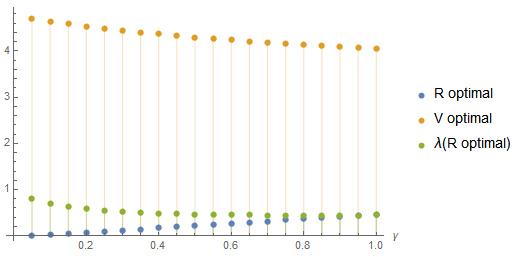
\includegraphics[width=0.6\textwidth]{Prob1_MaxProb/RVlambda_opt05.PNG}
	\caption{Optimal values of $R$ and $V(X)$ for fixed values of $F$ and $r$}
\end{figure}

We obtain that, although the optimal investment $R$ grows with exponent $\gamma$, the value function for the respective optimal $R$ decreases with exponent $\gamma$ (and in a different way from the decreasing of $\lambda(R)$). We get that the smaller value of $V(X)$ is approximately 4.05, corresponding to the optimal investment level $R=1$ and $\lambda(R)=0.45$ and the biggest value of $V(X)$ is approximately 4.69, corresponding to the optimal investment level $R=0.014$ and $\lambda(R)=0.05$
